
\section{From Introduction}

\begin{comment}
The document is organized as follows and motivated by the tasks
identified in the previous section. Each section is augmented with the
key area it contributes to.

\begin{itemize}
  
\item Section \ref{sec:definitions}: Definitions and Concepts: Develop
  a brief list of definitions that can be used to improve
  communication between different interdisciplinary groups while
  allowing them to use the same language.

\item Section \ref{sec:usecases}: Use Cases for Analytic Services:
  A compilation and organization of use cases focusing on analytic
  services including traditional statistical, AI/ML/DL, and emerging
  analytics application domains. It will help identifying the meta-
  and technical requirements.

\item Section \ref{sec:defining}: Defining and Finding Reusable Analytics
  Services. This section 
  will include the definition and conceptual architecture of reusable
  analytics services. This includes the following concerns that are
  organized as subsections.

 \begin{itemize}
 
    \item Section \ref{sec:fair}: Adaptation of the FAIR principle to
       supprt an Analytics Service FAIR Principle.

    \item Section \ref{sec:catalog}: Service Catalog: To communicate
      the existence of the services to others service registries can
      be used.

    \item Section \ref{sec:registry}: Service Registry: To communicate
      the the features of the services to others service registries
      can be used.

\end{itemize}

\item Section \ref{sec:federation} Service Analytics Federation: To leverage multiple
existing services federated services can be used to integarte them.

\item Section \ref{sec:data}: Data in Reusable Analytics Services:
  Here we explore a number of important issues related to data that is
  used by the analytics services.

\item Section \ref{sec:package}: Package Analytic Algorithms as
  Service Payloads: Here we explore how to package analytic algorithms
  with well-defined input and output parameters as service payloads
  that can be reusable, deployable, and operational across
  multi-cores, CPUs, and GPU computing platforms.

\item Section \ref{sec:interfaces}: Analytics Service Interfaces and
  Encapsulation: Here we explore a minimal set of services and their
  interfaces to be used as part of a generalized analytics
  framework. It includes to encapsulate the service payload with
  well-defined format, interface, and end-to-end access control for
  open and secure computing environment.
  
\item Section \ref{sec:resources}: Resource Management: Here we
  investigate and define a minimal set of resource management services
  and interfaces for application orchestration and workflow between
  processes.

\item Section \ref{sec:security}: Security Considerations in Reusable
  Analytics Services: Here we explore a number of important security
  considerations related to reusable analytics services.  

\item Section \ref{sec:outreach}: Outreach Activity: In our outreach
  activity we investigate the inclusion and collaboration with other
  interested parties.

\end{itemize}

\end{comment}

\section{Old use cases}

\subsection{Use Case Development Process}

To specify use cases for our analytics framework, we encourage
contributors to contact us and provide us with their high-level
descriptions of their use cases. The use cases should be focusing on
highlighting one or multiple aspects of the features related to
analytics frameworks. While inspecting the various features we intend
to collect and analyze them in various contexts that are relevant for
analytics users. The lessons learned from this analysis are to be
integrated into this document in order to formulate a comprehensive
vendor neutral analytics framework.  Use cases can be formulated in
various format but should include diagrams that make them easy to
comprehend as well as allowing the reader to extract the specific
analytical aspects. Such diagrams can include functional cross
diagrams, process diagrams and others.  Use cases should especially
address the use of metadata describing the functional and the data
related properties. This includes metadata related to time, space,
exchange/protocols, privacy, and security related aspects.  A
functional description of the use case is to be included as a
subsection called Functionalities and Activities. This section is
mirroring our experience with documenting use cases as part of the Big
Data Application Provider of NBDIF Reference Architecture. Hence, we
assume the following draft form for a use case:

\begin{description}
\item[Title:] 		Title of the use case
\item[Contributor:] 	The list co contributors
\item[Description:] 	One to two sentences about major functionalities and activities with respect to the sample cross-functional diagram
	
	\begin{description}
	\item[Cross-Functional Diagram:]
		Inclusion of a cross functional Diagram, alternatively other diagrams could be 			chosen.
	\item[Functionality Activities:]
	\begin{enumerate}
        \item Activity \#1 -- description ...
        \item ...
        \item Activity \#n -- description ...
    	\item Use Case Summaries
    \end{enumerate}
\end{description}
\end{description}

\begin{figure}[htb]
    \centering
    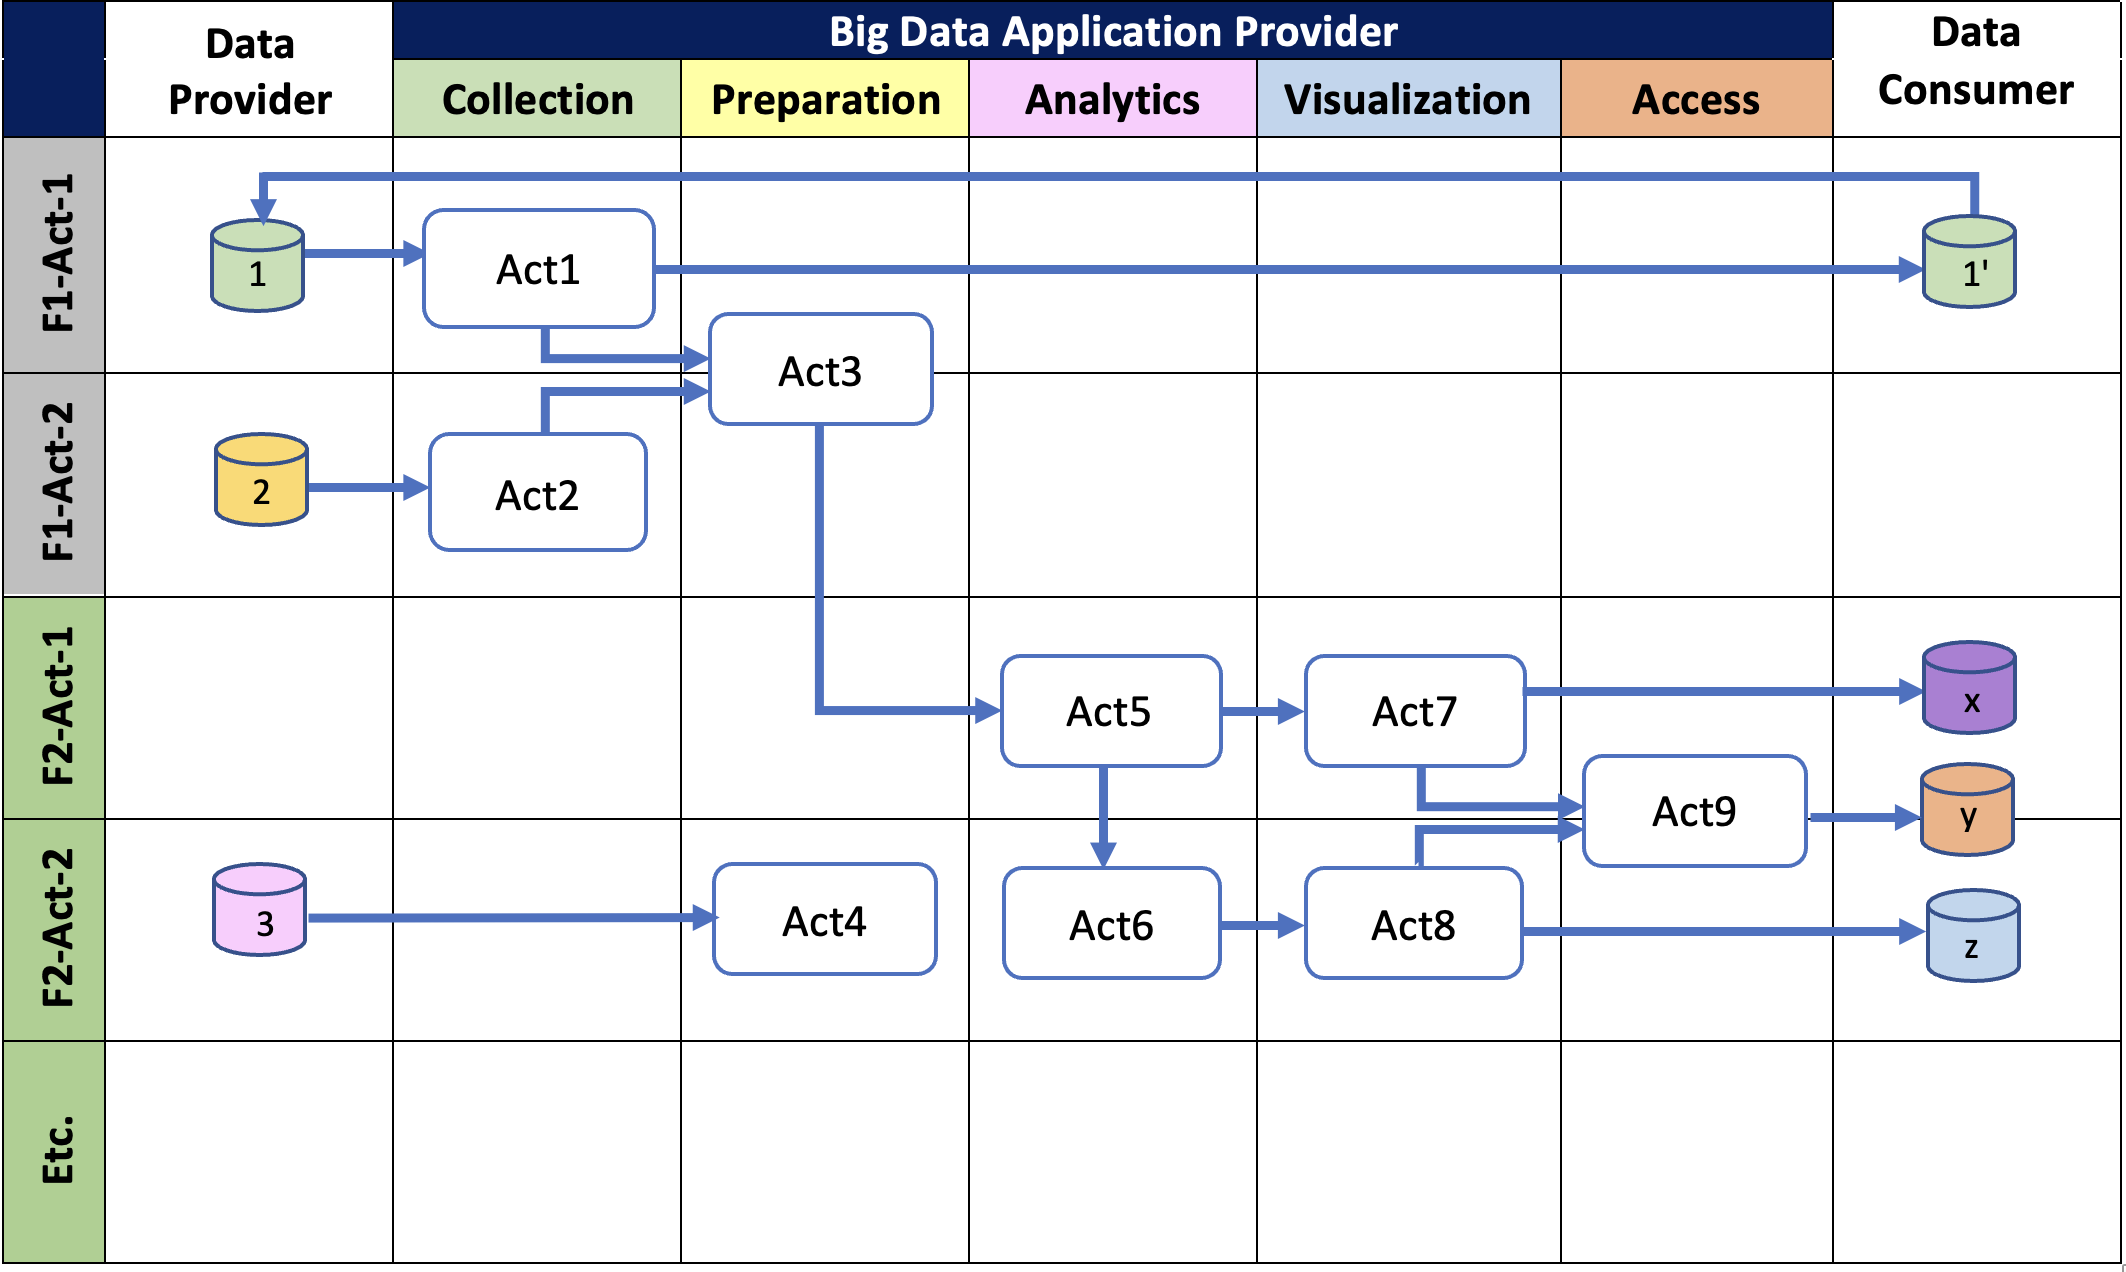
\includegraphics[width=1.0\columnwidth]{images/cross-functional-diagram.png}
    \caption{Cross-functional Diagram}
    \label{fig:cross-functional-diagram}
\end{figure}


Next, we will list use case summaries and if available point to specific publications on the NBDIF Web page that include more details. The expectation of this section is to
 
\begin{itemize}
\item	Provide an overview of use cases that motivate this document
\item	It will summarize requirements that we obtain from these use cases that influence how we proceed.
\end{itemize}

As a result, we identify how they fit into the workflow of data analytics. This includes the description of a subset of functionality that is used in general by data analytics.  In particular, it described the relationship between input and output of data analytics components and interfaces.  The use case summaries are expected to be available through the BigDataWG Web page and includes currently the following examples:

\begin{enumerate}
\item	\href{https://bigdatawg.nist.gov/_uploadfiles/M0701_v1_2020102001.docx}{M0701} -- Use case template \cite{nist-usecase-template}
\item	\href{https://bigdatawg.nist.gov/_uploadfiles/M0702_v1_2020102002.pdf}{M0702} -- Numeric weather prediction \cite{nist-wrf}
\item	\href{https://bigdatawg.nist.gov/_uploadfiles/M0703_v1_2020102003.pdf}{M0703} -- HVAC Heat ventilation and air conditioning \cite{nist-hvac}
\end{enumerate}


